\chapter{Desarrollo del proyecto\label{sec:disenho}}

Para la realización de este trabajo se han tomado dos  de las tecnologías expuestas en el capítulo anterior. %REFERENCIA CAPITULO ANTERIOR
La finalidad de esto es poder trabajar experimentalmente/empíricamente con dos tecnologías y una vez realizado todo el trabajo práctico proceder a evaluar las características de cada tecnología y la comparativa entre ellas.

Es por ello que este capítulo se estructura en los dos puntos siguientes: sensores de Bragg y sensores IMU. Dentro de cada punto se detalla toda la información necesaria para la implementación de cada uno de los sistemas.\cite{SilviaTFM}

\begin{itemize}
	\item {Sensores FBG}
	\item {IMU}
\end{itemize}

%------FFFFFFBBBBBBGGGGGG------
\section{Sensores FBG}
\label{sec:FBG3}
Introducción breve del guante, que tecnologias implica.


Resumen fibras de Bragg 
¿Qué es una fibra FBG?
¿POrque se utilizan?

El procesado de las señales resultantes se realiza mediante labview. 

%--Marco conceptual
\subsection{Marco conceptual}
\label{sec:mc3FBG}

Este apartado tiene por finalidad realizar una clara exposición de los conceptos teóricos fundamentales para la comprensión del diseño llevado a cabo.

\begin{itemize}
	\item \textbf{Fibra óptica}
	
	Cómo se propaga la luz en ella.
	
	partes de la fibra.
	
	Tipos de emisores (LED Laser).
	
	Receptores.
	
	Conectores.
	
		\item \textbf{Redes de difracción de Bragg}
		
	Funcionamiento y sensibilidad
		\item \textbf{Polidimetilsiloxano (PDMS)}
		
	Material empleado para embeber las FBGs.
	
		
\end{itemize}
 
%--Desarrollo del prototipo
\subsection{Desarrollo del prototipo}
\label{sec:prot3FBG}
%[Esta parte de desarrollo del proyecto parte de otro trabajo. Aquí mencionar algo que diga el trabajo de Silvia y mencionar la en la bibliografía.]

La realización del primer desarrollo se origina a partir de un trabajo realizado con anterioridad en el grupo de investigación de la universidad\cite{SilviaTFM}. Se mejora el soporte físico(hardware) y se desarrolla un nuevo programa con un interfaz de usuario simple e intuitivo.

El prototipo consiste en un prototipo técnico y funcional de un guante, con sensores de FBG embebidos en PDMS. 
 
\subsubsection{Materiales}
En este apartado se disponen brevemente los componentes utilizados para el 
\begin{figure}[H]
	\centering
	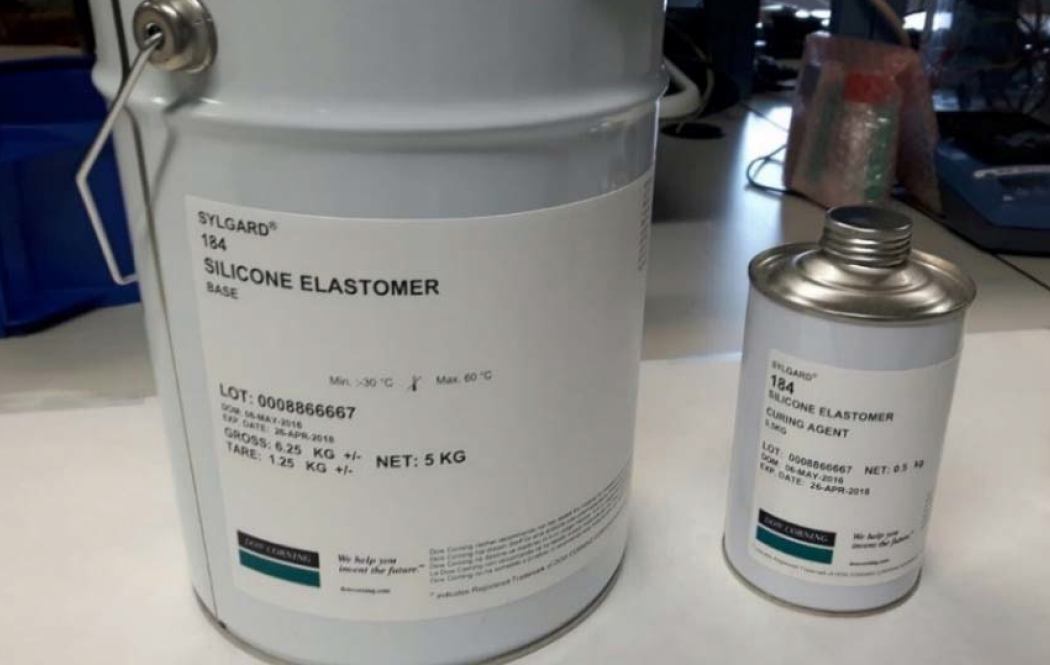
\includegraphics[width=0.75\textwidth]{./img/PDMS}
	\caption{PDMS: Elastómero y agente de cura.} \label{fig:pdms}
\end{figure}



\subsubsection{Proceso de fabricación del soporte físico}
%Elaboración
Para que sea más cómoda la explicación del proceso de elaboración del prototipo se divide este en tres partes: modelado 3D, fabricación del guante y montaje de prototipo completo.

\begin{itemize}
	\item \textbf{Modelado 3D - Configuración 3D}
	
	Esta actividad comprende el diseño del molde con el que se fabrica el guante y de la caja contenedora de todo el cableado.
	Para poder producir el guante de PDMS es necesario tener un molde donde verter la disolución para darle la forma deseada. Gracias a las versatilidad de diseño que ofrece la impresión 3D se realiza con este proceso de manufactura el molde (véase figura \ref{fig:molde}). 
\begin{figure}[H]
	\centering
	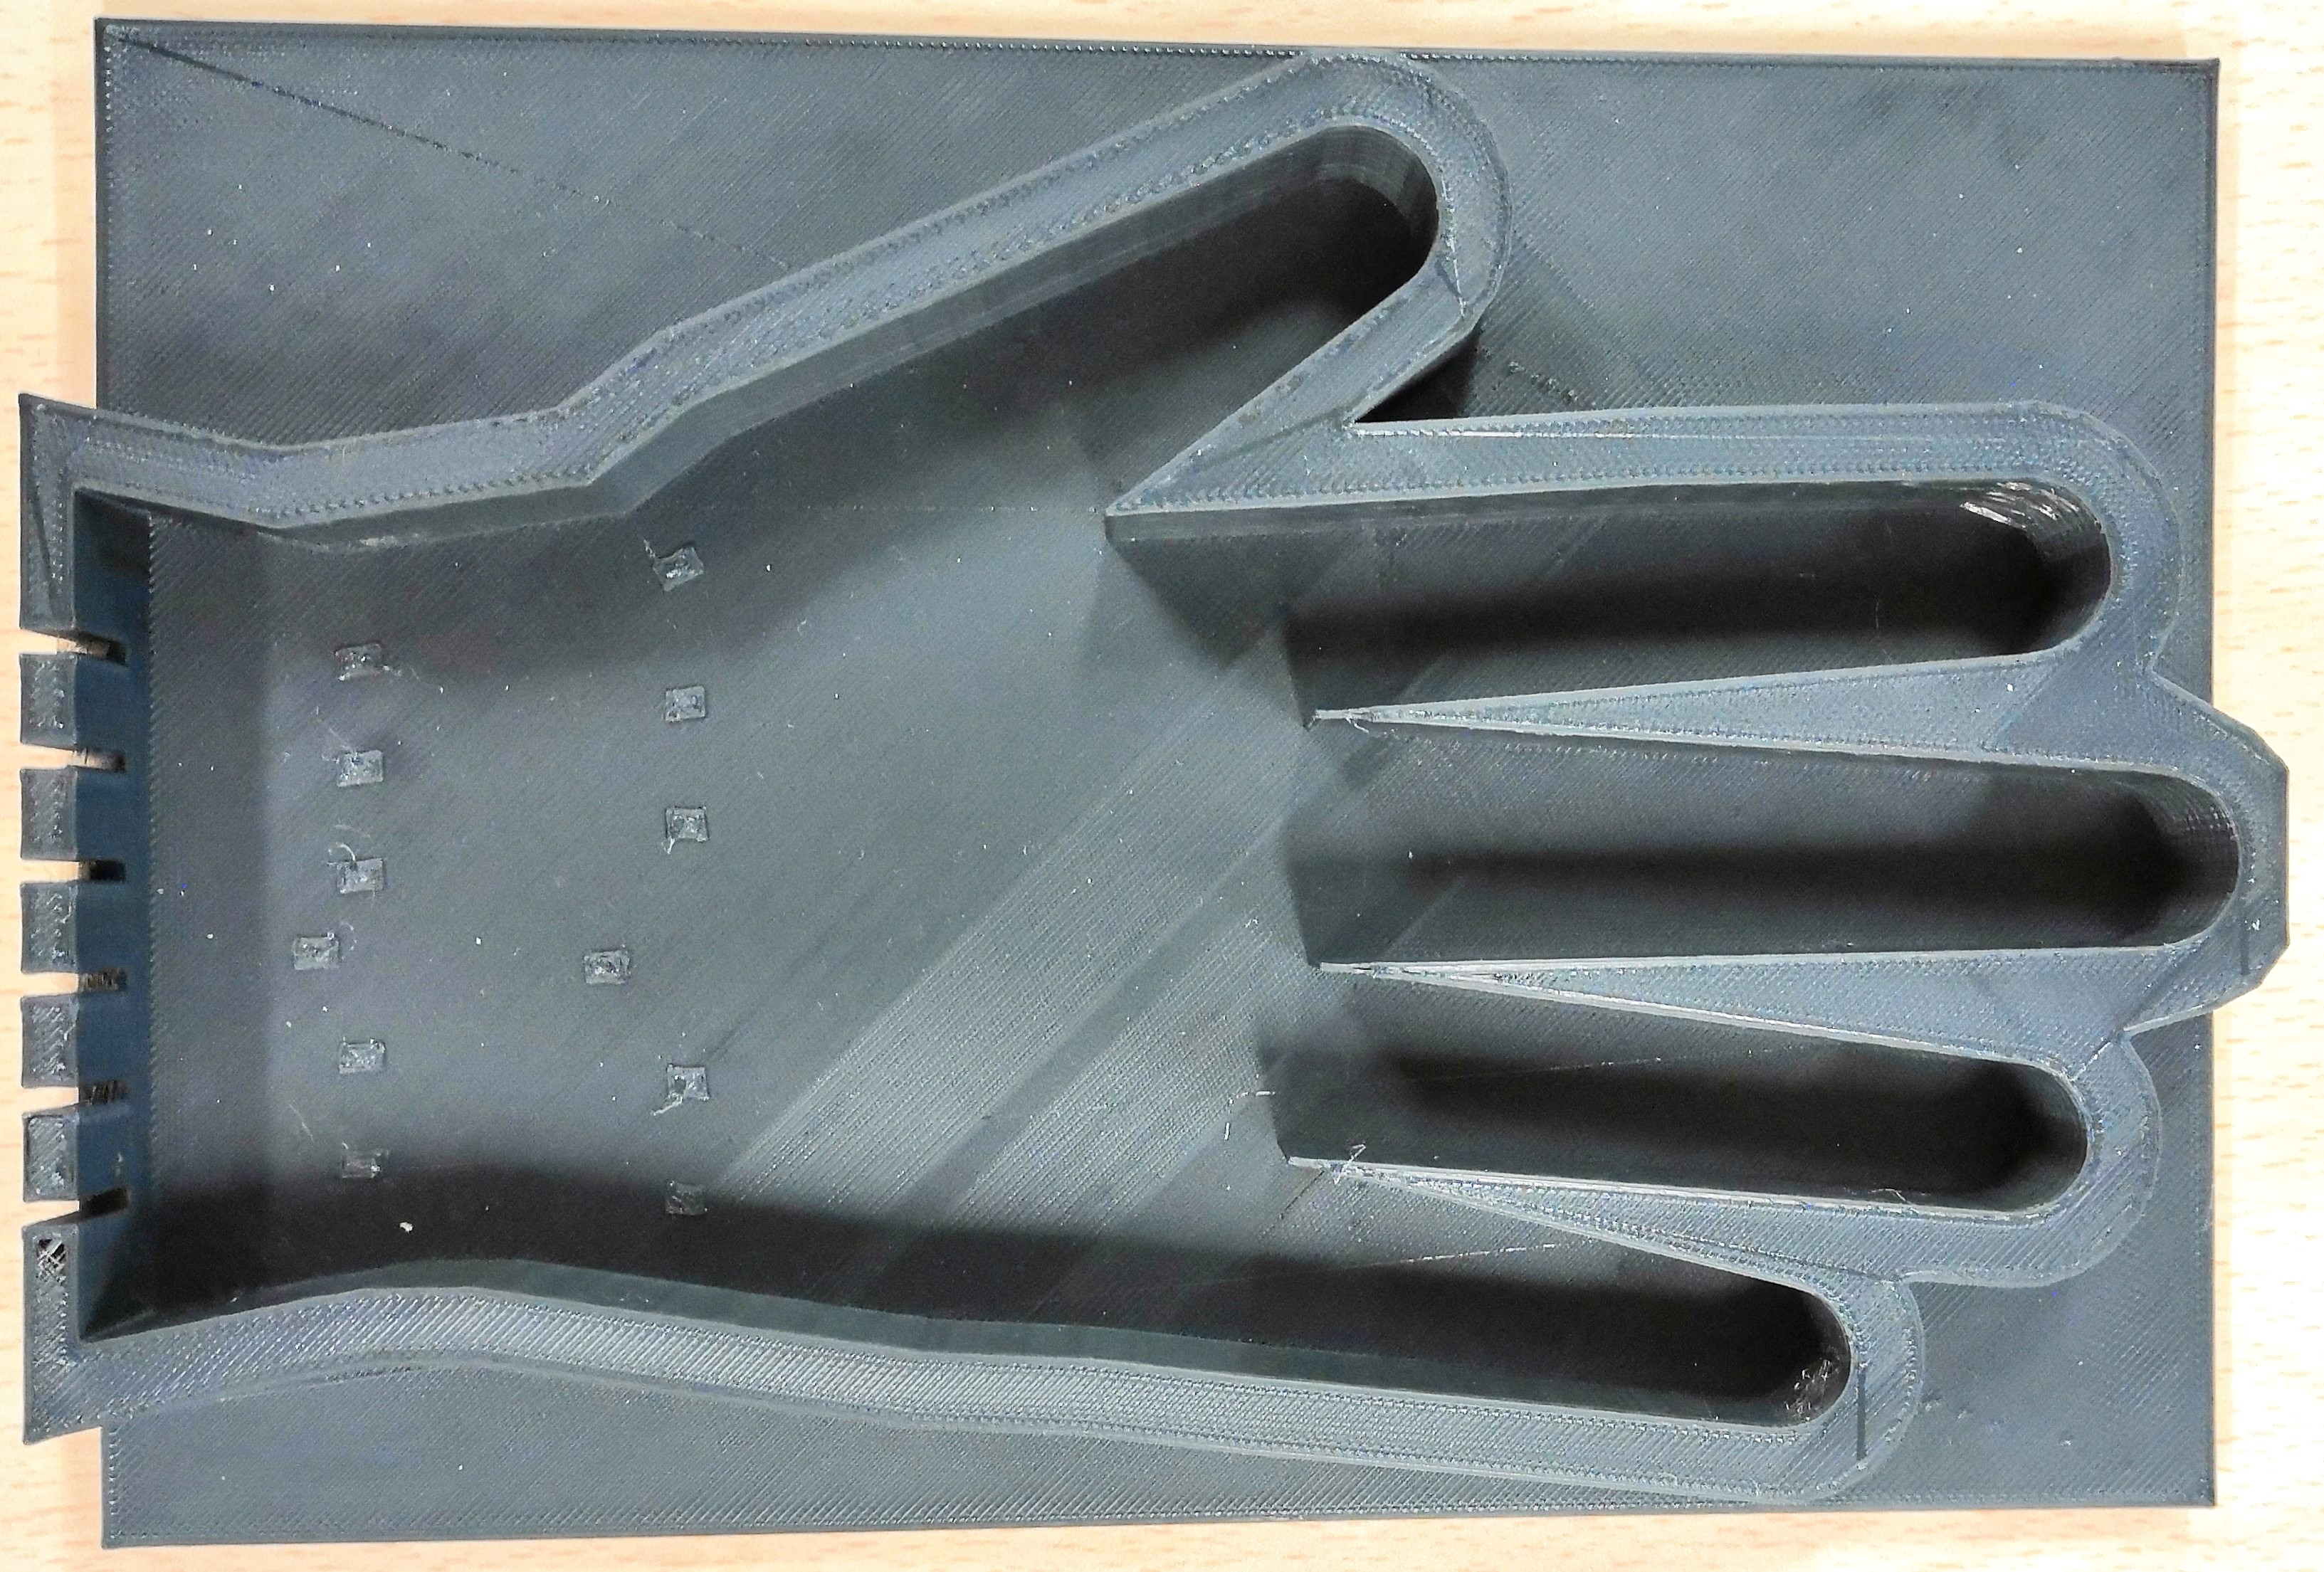
\includegraphics[width=0.5\textwidth]{./img/molde1}
	\caption{Molde} \label{fig:molde}
\end{figure}

	
 
	\item \textbf{Fabricación del guante}
	
	Para el proceso de fabricación del guante se necesitan ..................
	
	\begin{enumerate}
		\item Preparar mezcla PDMS (35g de polímero y 3.5g de agente de curación). Primero el
		elastómeto y después agente de curación.
		\item Revolver la mezcla durante al menos 4 minutos.
		\item Se deposita el PDMS y se colocan las fibras en el molde
		\item Se introduce en un horno de vacío para eliminar las burbujas durante 20 minutos, sin aplicar
		temperatura.
		\item Meter el molde en el horno (4h y media a $-55\,^{\circ}\mathrm{C}$). Dejar un poco más.
		\item Desmoldar.

	\end{enumerate}
	
	
	\item \textbf{Montaje completo}
	
	asdf
	
\end{itemize}

asdf



-------------------------------------------------------////
\begin{table}[H]
	\centering
	\begin{tabular}[t]{|r|c|}
		\hline
		 & Longitud de onda del sensor\\
		\hline
		\hline
		Dedo pulgar & 1512 nm \\
		\hline
		Dedo índice & 1520 nm \\
		\hline
		Dedo corazón & 1528 nm \\
		\hline
		Dedo anular & 1536 nm \\
		\hline
		Dedo meñique & 1544 nm \\
		\hline
		Muñeca & 1556 nm \\
		\hline
	\end{tabular}
	\caption{Tabla longitud de cada sensor FBG}
	\label{tabla:medidas 80 cm}
\end{table}
-------------------------------------------------------////
\begin{table}[H]
	\centering
	\begin{tabular}[t]{|r|c|}
		\hline
		& Longitud de onda del sensor\\
		\hline
		\hline
		Dedo pulgar & 1532 nm \\
		\hline
		Dedo índice & 1548 nm \\
		\hline
		Dedo corazón & 1560 nm \\
		\hline
		Dedo anular & 1568 nm \\
		\hline
		Dedo meñique & 1576 nm \\
		\hline
		Muñeca & ---15?? nm--- \\
		\hline
	\end{tabular}
	\caption{Tabla longitud de cada sensor FBG}
	\label{tabla:medidas 80 cm}
\end{table}

Para determinar la valid


\subsubsection{Funcionamiento}
asdf

\begin{figure}[H]
	\centering
	\includegraphics[width=1\textwidth]{./img/interfazSM}
	\caption{Interfaz del programa de labview.}
	\label{fig:interfaz}
\end{figure}

%------IIIIIIMMMMMMUUUUUU------
\section{IMU}
\label{sec:IMU3}
asdf

\subsection{Marco conceptual}
\label{sec:mc3IMU}
asdf

\subsection{Desarrollo del prototipo}
\label{sec:prot3IMU}
asdf

\subsubsection{Materiales}
asdf


\subsubsection{Elaboración/Proceso de fabricación}
asdf

\subsubsection{Funcionamiento}
asdf




\section{---------------}

ME PLENTEO LA POSIBILIDAD DE DIVIDIR EL CAPITULO 3 EN CAPITULO 3 Y 4.


----------------------------------------------------------------------------------------------------------------------------------------------------------------------------------------------------------------------------------------------------------------------------------------------------------------------------------------------------------------------------------------------------------------------------------------------------------------------------------------------------------------------------------------------------------------------------------------------------------------------------------------------------------------------------------------------------------------------------------------------------------------------------------------------------------------------------------------------------------------------------------------------------------------------------------------------------------------------------------------------------------------------------------------------------------------------------------------------------------------------------------------------------------------------------------------------------------------------------------------------------------------------------------------------------------------------------------------------------------------------------------------------


\section{---------------}















En este capítulo se detalla la metodología empleada para el diseño del sistema adaptado al contexto en el que se aplica. Se describe cada uno de los componentes que forman parte del sistema de medición así como el procesado posterior de los datos para obtener la distancia entre pasos(Matlab\textsuperscript{\textregistered}). En el diseño intervienen sensores inerciales (Xsens Technologies B.V, The Netherlands) y se propone el diseño de un sensor de ultrasonido de bajo coste basado en la tecnología Arduino. 


\section{Sistema de medida}
En la Figura \ref{fig:esquema} aparece representado un esquema general de la metodología empleada. Mediante el sensor de ultrasonidos se obtiene la distancia D1 y con los sensores inerciales se obtiene la distancia D2 aplicando a cada una de las señales el procesado que se detallará en posteriores apartados.


Por tanto, el diseño del sistema puede descomponerse en dos niveles de jerarquía  (ver Figura \ref{fig:esquemaniveles}). El primero de ellos, a más bajo nivel, es el diseño del sensor de ultrasonidos y la obtención de las señales necesarias para el cálculo de cada una de las distancias de ambos sensores. El segundo de los niveles es el correspondiente al de la sincronizcación y post-procesado de los datos para determinar la distancia entre pasos.

 Con el  post-procesado de las señales obtenidas por cada uno de los sensores se obtendrán las distancias D1 y D2 que permitirán el cálculo de la distancia objetivo mediante la ecuación \ref{eq:distancia} (Teorema de Pitágoras).

\begin{equation}\label{eq:distancia}
Dist.sep.pasos = \sqrt{D1^2 + D2^2}
\end{equation}


En los siguientes apartados se especifican cada uno de los componentes que intervienen en el sistema. 
\section{Sensores inerciales}
\subsection{Principio de funcionamiento}

Un sistema de referencia inercial se trata de un sistema de referencia regido por las leyes de movimiento de Newton. Por tanto, un sensor capaz de medir valores respecto a dicho sistema de referencia es lo que se conoce como un sensor inercial.

Una unidad inercial o IMU (Inertial Magnetic Unit) es un dispositivo que se compone de tres giróscopos (para determinar la orientación), tres acelerómetros y un reloj que permite asignar tiempo a los valores medidos por los sensores inerciales. Dichas unidades inerciales presentan tres ejes y cada uno de ellos presenta un acelerómetro y un giróscopo.

Por tanto, la información que se recoge de las unidades inerciales son aceleraciones lineales, velocidades angulares y tiempo común para los tres ejes que llevan dicha información de aceleración y velocidad angular (ver Figura \ref{fig:Imu}). 


El tiempo requerido para la implementación del sistema de medida puede influir en la marcha de los pacientes y por tanto en la obtención de los parámetros \cite{begona}. Los sensores inerciales utilizados permiten realizar las mediciones de una manera sencilla y rápida lo cual resulta beneficioso en el contexto ambulatorio tanto para los pacientes como para el personal sanitario



\subsection{Sensores inerciales propuestos}
Los sensores inerciales utilizados para el sistema son el modelo MTw Awinda (Xsens Technologies B.V, The Netherlands) pueden verse representados en la Figura \ref{fig:sensor_XSENS}



Su tamaño es de 47 x 30 x 13mm y 16g de peso por lo que puede definirse como un sistema compacto y ergonómico que será de utilidad para el sistema propuesto en este trabajo. Dispone de unas bandas de sujeción que permiten colocar el sensor en el lugar necesario y por tanto dota de versatilidad al diseño. 

Además, se incluye un software de captura que resultará útil para obtener las señales para su posterior procesado. La comunicación de los sensores con el software emplea un protocolo propietario que aparece representado en la Figura \ref{fig:protocolo}.

	
\section{Sensor de ultrasonido}

\subsection{Principio de funcionamiento}
Un sistema de ultrasonidos tiene como principio de funcionamiento el fenómeno físico por el cual recibe ese nombre, las ondas de ultrasonidos.

Se envía un pulso de 40 KHz que incide sobre un obstáculo y se recibe con un retardo que se corresponde con el tiempo que tarda la onda desde que se envía hasta que se recibe, es decir el Time of Flight" (ToF). Por tanto, puede hallarse la distancia mediante la 

	 En la Figura \ref{fig:ultr} se observa dicho funcionamiento.

La distancia entre dos puntos puede hallarse mediante la ecuación \ref{eq:dis_ult}
	\begin{equation}\label{eq:dis_ult}
	D = (ToF/2)V_{sonido}
	\end{equation}
	
Una alternativa al sistema de ultrasonidos es usar la tecnología de infrarrojos. Su principal ventaja es su rápida respuesta y por ello resulta beneficioso para aplicaciones en tiempo real como pueden ser los sensores de proximidad. La principal desventaja es que presentan no linealidades procedentes de su dependencia con la superficie de reflexión. Es necesario un conocimiento a priori de las características de dispersión, absorción etc. del material sobre el que incide la onda emitida para poder realizar una medida de distancia correcta. 

Teniendo en cuenta las características de ambos sensores, se decidió que el sensor más apropiado para la aplicación clínica de este trabajo es el sensor de ultrasonidos, ya que su coste no es elevado y su resolución y su latencia son aceptables. Se ha descartado el uso de un sensor de infrarrojos, por un lado, porque la velocidad no es un factor crítico y por otro lado, realizar una medida de distancia con este tipo de sensores supone la necesidad de conocer a priori el material del calzado de cada paciente o añadir una superficie con un material concreto en uno de los zapatos del paciente lo cual hace que el diseño resulte menos ergonómico. Finalmente añadir que aunque existen sensores de infrarrojo basados en la medida de desfase que podrían utilizarse como sensores de distancia, su precio es realmente elevado para las características necesarias en este trabajo \cite{infra}
	

\subsection{Sensor de ultrasonido propuesto}\label{su}

	El principal objetivo en el diseño del sensor es optimizar el compromiso entre bajo coste y precisión. En la Figura \ref{fig:sensor_ultrasonido} puede verse el prototipo del sensor. Este primer prototipo está compuesto por un sensor de ultrasonidos HC-SR04 (1), un módulo Bluetooth (2) para el envío de datos a un PC, una placa Arduino UNO (3) para el procesado de la información del sensor, y la alimentación mediante una pila recargable de 9V (4) para dotar de autonomía al sistema.

 \begin{figure}[H]
 	\centering
 	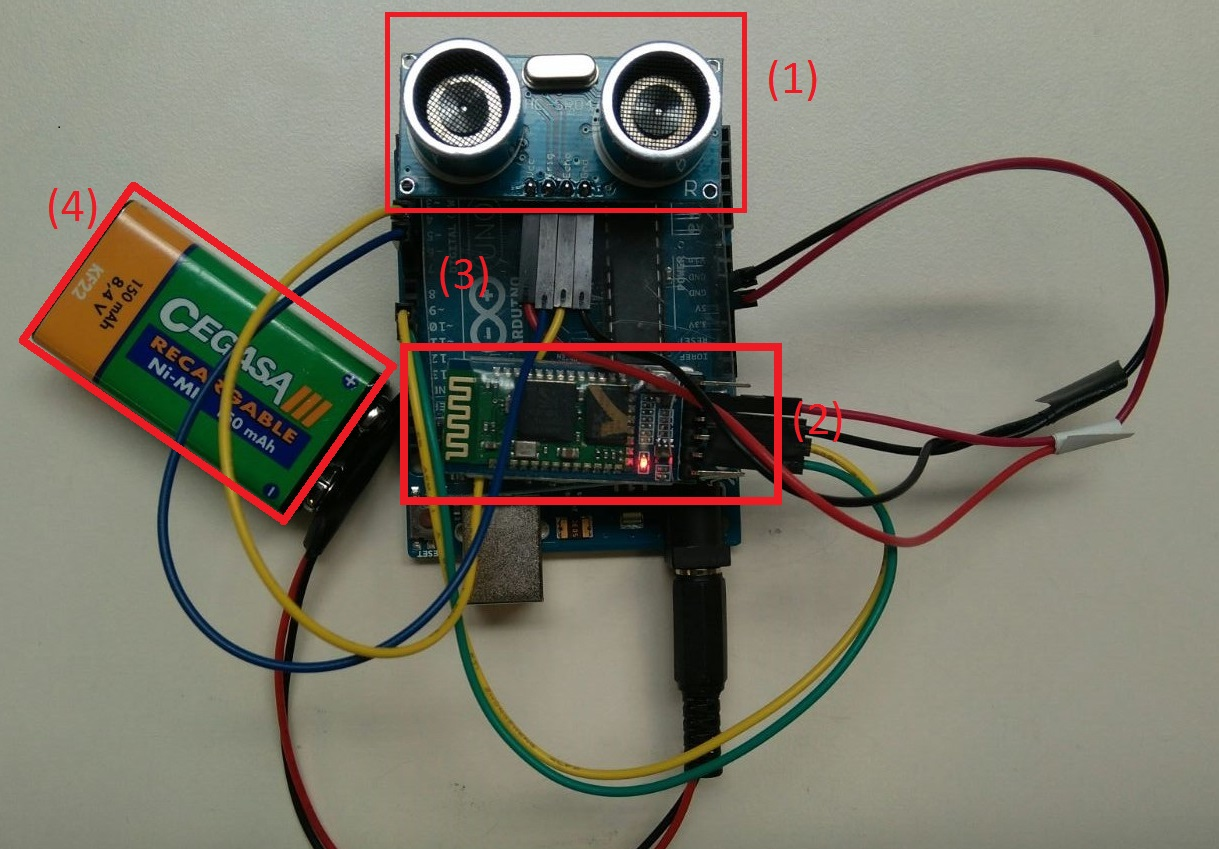
\includegraphics[width=0.7\textwidth]{./graphics/sensor}
 	\caption{Prototipo de sensor de ultrasonidos} \label{fig:sensor_ultrasonido}
 \end{figure}

	\subsubsection{Conexionado del sensor}
		El conexionado del prototipo (apartado \ref{su}), aparece representado de manera esquemática en la Figura \ref{fig:conexionado} con el fin de clarificar las conexiones. En un futuro diseño más compacto, la placa utilizada, así como algunos de los componentes, serán modificados manteniendo el enfoque de bajo coste, ergonomía y precisión. Por ello las conexiones podrán ser modificadas según sea necesario.
		
		 
		\begin{figure}[H]
			\centering
			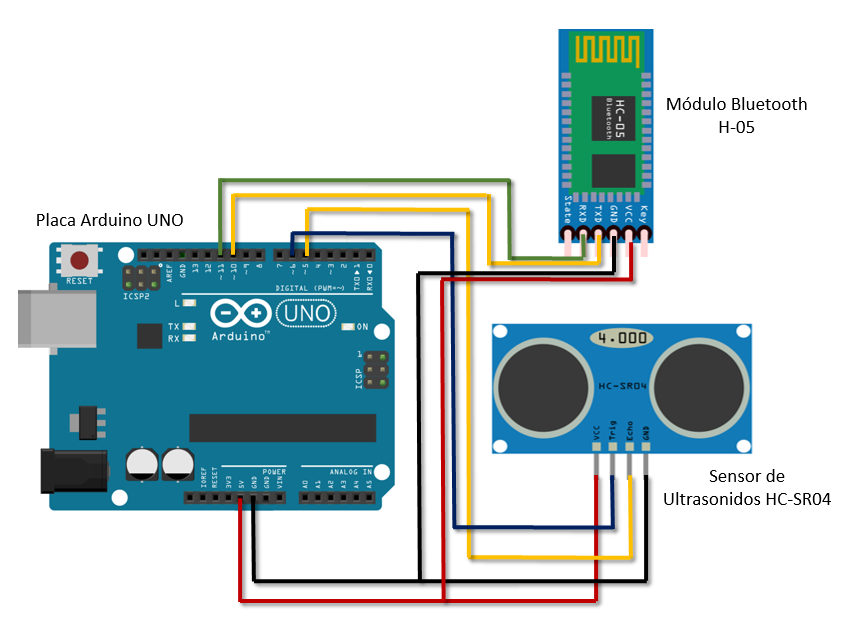
\includegraphics[width=0.7\textwidth]{./graphics/conexionado}
			\caption{Esquema de conexión del sensor de ultrasonido} \label{fig:conexionado}
		\end{figure}
		
	\subsection{Comunicación del sensor}
	
		\subsubsection{Bluetooth}
		
		Para el envío de la información de distancia desde la placa Arduino hasta el PC donde se van a procesar los datos, se ha elegido el módulo comercial Bluetooth H-05 que aparece representado en la Figura \ref{fig:bluetooth}.
		
	
			 \begin{figure}[H]
			 	\centering
			 	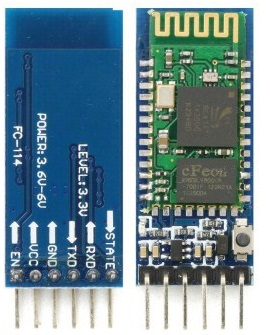
\includegraphics[width=0.25\textwidth]{./graphics/bluetooth}
			 	\caption{Módulo Bluetooth HC-05} \label{fig:bluetooth}
			 \end{figure}
			 
		Dicho módulo se comunicará con un dongle USB 4.0 en el PC ya que éste no dispone de interfaz Bluetooth de serie (ver Figura \ref{fig:dongle}). Además es compatible con estándares anteriores (2.0, 3.0) por lo que resulta apropiado para el diseño.
		
		
		\begin{figure}[H]
			\centering
			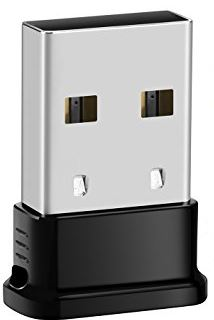
\includegraphics[width=0.15\textwidth]{./graphics/dongle}
			\caption{Dongle Bluetooth 4.0 WhiteLabel} \label{fig:dongle}
		\end{figure}
			
		\subsubsection{Software de captura}
		
		En este trabajo se ha diseñado un software de captura (Figura \ref{fig:software}) para la obtención de los datos de distancia suministrados por el sensor.
		

		Las funcionalidades principales de este software son:
		\begin{enumerate}
				\item Creación del interfaz Bluetooth para la comunicación con Matlab. 
				\item Representación de los datos recogidos en tiempo real.
				\item Posibilidad de guardar los datos en un archivo.
				\item Posibilidad de cargar un archivo y representarlo offline.
		\end{enumerate}
	
		
\section{Procedimiento de medida}		

\subsection{Set-up de medida}
Para demostrar la viabilidad del sistema en cuanto a su capacidad para medir la distancia de separación entre pasos,se proponen dos set-ups que consisten en establecer unas marcas en el suelo a una distancia conocida para así, una vez realizado el procesado de las señales, poder determinar si los resultados son correctos. El primer set-up consta de una medida de paso de 43 cm (ver Figura \ref{fig:setup_43}) y el segundo para una de 80.5 cm (ver Figura  \ref{fig:setup_80} ). 

\begin{figure}[H]
	\centering
	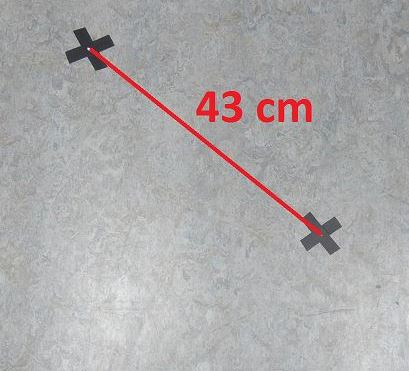
\includegraphics[width=0.55\textwidth]{./graphics/setup_43}
	\caption{Set-up de medida de un paso de 43 cm} \label{fig:setup_43}
\end{figure}

\begin{figure}[H]
		\centering
		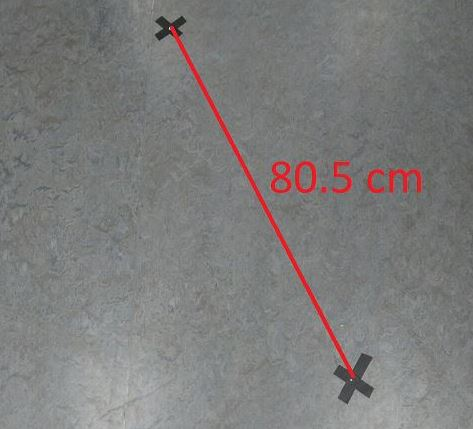
\includegraphics[width=0.55\textwidth]{./graphics/setup_80}
		\caption{Set-up de medida de un paso de 80.5 cm} \label{fig:setup_80}
\end{figure}
	
Este montaje permitirá el poder medir un la distancia de un paso para verificar que el tanto el funcionamiento como el procesado con correctos. Se dejará como línea futura el poder realizar el procesado de forma automática y para varios pasos. Para realizar las medidas se ha colocado un sensor inercial en cada pie y el sensor de ultrasonidos en el tobillo según se representa en la Figura \ref{fig:colocar} y \ref{fig:paso}. 
\begin{figure}[H]
	\centering
	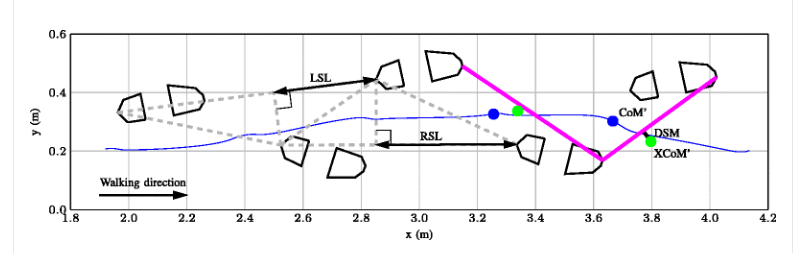
\includegraphics[width=0.55\textwidth]{./graphics/Medida}
	\caption{Colocación de los sensores para la medida} \label{fig:colocar}
\end{figure}
\begin{figure}[H]
	\centering
	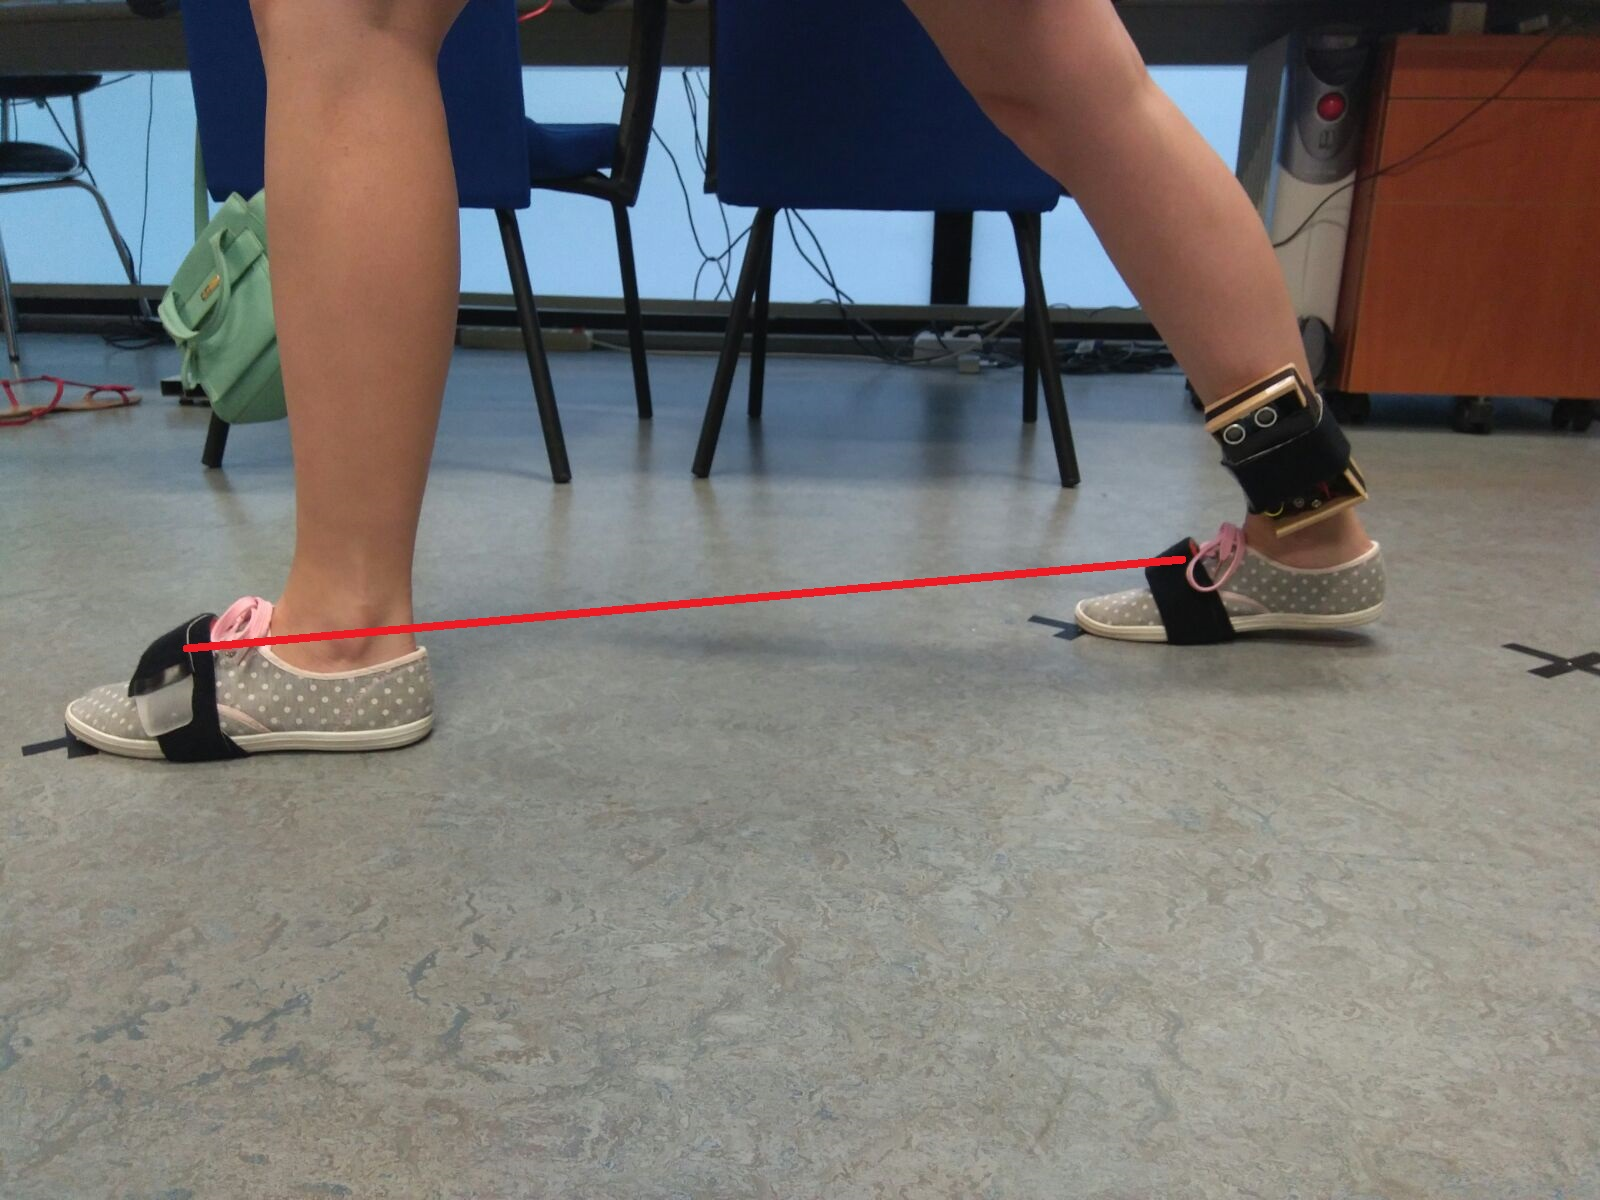
\includegraphics[width=0.65\textwidth]{./graphics/paso}
	\caption{Ejemplo de paso para la medida} \label{fig:paso}
\end{figure}


\subsection{Captura de datos}

Para llevar a cabo la medida se colocará un sensor inercial en cada pie y el sensor de ultrasonidos en uno de ellos. A continuación, se capturarán los datos de los sensores inerciales mediante el software específico MTManager de Xsens y los datos del sensor de ultrasonido mediante el software realizado con MATLAB\textsuperscript{\textregistered} 


\subsection{Sincronización}
Una de las etapas clave del diseño del sistema a tiempo real es el de la sincronización de ambos sensores. En este trabajo, para una demostración de funcionamiento, el procesado de las señales de ambos sensores se realizará por separado de forma que se pueda demostrar el funcionamiento del sistema y se dejará como línea futura de investigación la sincronización. 

Se pretende conseguir una lectura de los datos del sensor de ultrasonido en el PC con un tiempo de muestreo constante. En este punto del trabajo se encuentran dificultades con la forma en que Matlab lee los datos. Los datos enviados por el sensor son constantes pero la lectura hace ese tiempo variable. Si se consigue un tiempo constante, mediante procesados como la interpolación podría sincronizarse con los sensores inerciales. Además, debido a que se utilizan dos programas de captura, es necesario establecer un inicio que se considere como principio tanto para las señales de los sensores inerciales como el de ultrasonidos. 


\subsection{Obtención de distancia}
Para la obtención de la distancia de separación entre pasos existen tres scripts realizados con la herramienta software Matlab\textsuperscript{\textregistered}

Mediante un software en Matlab\textsuperscript{\textregistered} se cargan las señales y se realiza el post-procesado para obtener cada una de las distancias que van a permitir la obtención de la distancia de separación entre pasos.

Se procesará el cálculo de las distancias deseadas de los sensores inerciales y del de ultrasonido y dichas informaciones se utilizarán para la obtención de la distancia de separación entre pasos.

\subsubsection{Sensores inerciales}

	
	Para la obtención del dato de distancia a partir de las señales proporcionados por los sensores inerciales es necesario tener en cuenta que la distancia se recorre en el plano en el que se produce el avance, que es este caso es el plano XY.

Para obtener la posición en este plano a partir de la aceleración en los tres ejes XYZ proporcionada por los sensores inerciales, es necesaria una doble integración.Posteriormente se elimina la deriva existente en las señales debido a esta integración. A continuación se describen los cálculos realizados

\begin{itemize}
	
	\item{\textbf{Obtención de la velocidad}}
	
		Se realiza una primera integración de la aceleración en el eje X y en el eje Y de donde se obtiene la velocidad tal y como aparece en la Figura \ref{fig:vel_no_corr}
	 \begin{figure}[H]
	 	\centering
	 	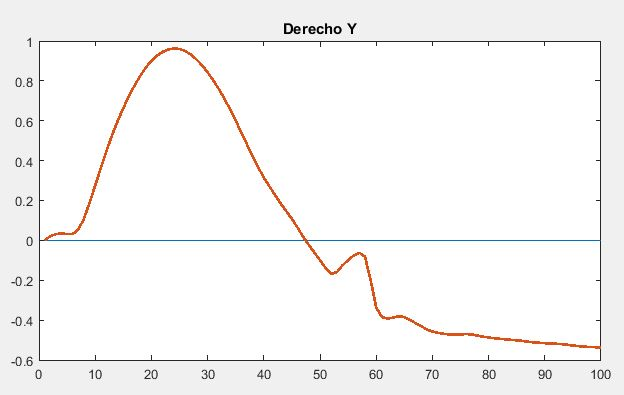
\includegraphics[width=0.81\textwidth]{./graphics/vel_no_corr}
	 	\caption{Ejemplo de deriva en la señal} \label{fig:vel_no_corr}
	 	
	 \end{figure}
 
	\item{\textbf{Obtención de la velocidad sin deriva}}	
	
En el instante de inicio y fin del paso, cuando el pie permanece apoyado, la velocidad debe ser cero.. Para lograr eliminar la deriva en la señal se propone utilizar la ecuación de la recta (color morado) que aparece en la Figura  \ref{fig:vel_no_corr_rect} . Dicha recta entre dos puntos A(a1, a2) y B(b1,b2) se difine mediante la ecuación \ref{eq:recta}
	
	\begin{equation}\label{eq:recta}
	y = (\frac{b_{2}-b_{1}}{a_{2}-a_{1}})*(x-a_{1})+b_{1}
	\end{equation}
	
	;donde:
	\begin{itemize}
		\item b2: coordenada y del último punto escogido (B)
		\item b1: coordenada x del último punto escogido (B)
		\item a2: coordenada x del primer punto escogido (A)
		\item a1: coordenada y del primer punto escogido (A)

	
	\end{itemize}


		 \begin{figure}[H]
		 	\centering
		 	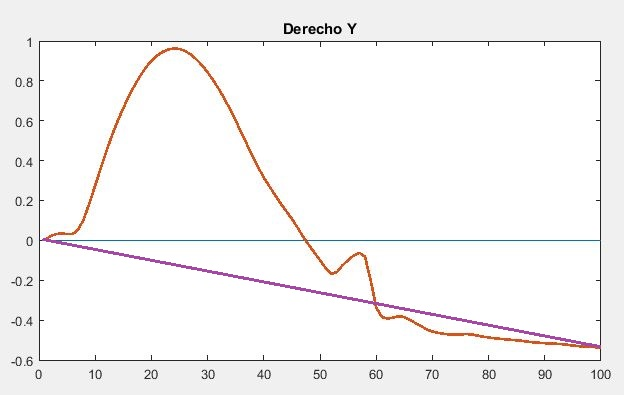
\includegraphics[width=0.8\textwidth]{./graphics/vel_no_corr_deriva}
		 	\caption{Recta para la corrección de la deriva} \label{fig:vel_no_corr_rect}
		 	
		 \end{figure}
De esta forma restando a la señal de velocidad la recta calculada, el resultado es el que aparece en la Figura \ref{fig:corregida} donde se representa la velocidad sin deriva.

	
		 \begin{figure}[H]
		 	\centering
		 	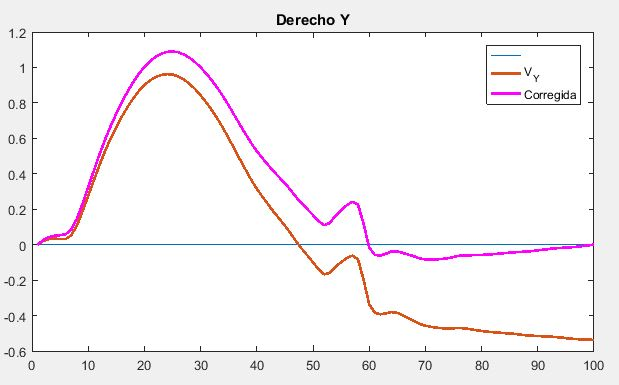
\includegraphics[width=0.8\textwidth]{./graphics/corregida}
		 	\caption{Ejemplo eliminación de la deriva} \label{fig:corregida}
		 \end{figure}


	\item{\textbf{Obtención de distancia D2 de sensores inerciales}}

	
	Una vez corregida la deriva en las velocidades X e Y de los sensores izquierdo y derecho en necesaria una segunda integración para hallar la posición en cada uno de los ejes. A continuación se representa la posición en el eje X con respecto al eje Y para calcular la distancia total en el plano XY (ver Figura \ref{fig:posi})
	\begin{figure}[H]
		\centering
		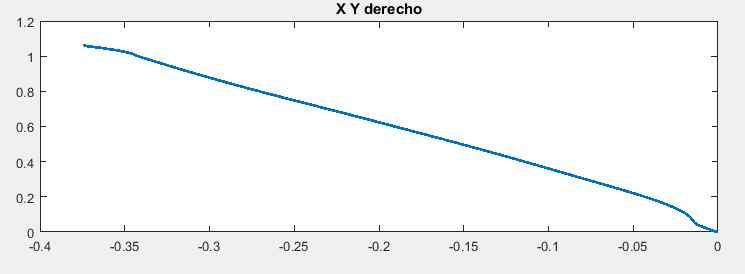
\includegraphics[width=1\textwidth]{./graphics/posi}
		\caption{Ejemplo eliminación de la deriva} \label{fig:posi}
		
	\end{figure}
	
	Para el cálculo de la distancia será necesario la eliminación de la deriva en la posición.
	
	La distancia (D2) ahora será la distancia entre los puntos inicial y final de la Figura \ref{fig:posi}, una vez corregida la deriva, que se calculará mediante la ecuación \ref{eq:pos}
		\begin{equation}\label{eq:pos}
		Distancia = \sqrt{(b_{1}-a_{1})^{2}+(b_{2}-a_{2})^{2}}
		\end{equation}
		\begin{equation}\label{eq:punto2}
			B = [b_{1},b_{2}]	
		\end{equation}
		\begin{equation}\label{eq:puntos1}
			A = [a_{1},a_{2}]
		\end{equation}
		;donde:
		\begin{itemize}
		\item b2: coordenada y del último punto escogido (B)
		\item b1: coordenada x del último punto escogido (B)
		\item a2: coordenada x del primer punto escogido (A)
		\item a1: coordenada y del primer punto escogido (A)
		\end{itemize}
\end{itemize}



\subsubsection{Sensor de ultrasonido}

	Previamente a la obtención de la distancia que se desea obtener usando el sensor de ultrasonido, se realiza una comprobación del correcto funcionamiento tanto del dispositivo como del envío de datos al PC vía Bluetooth. Inicialmente se realizan medidas con el sensor en estático. Para ello se propone el set-up de medida que aparece representado en la Figura  \ref{fig:ultrasonido}.
		
		 \begin{figure}[H]
		 	\centering
		 	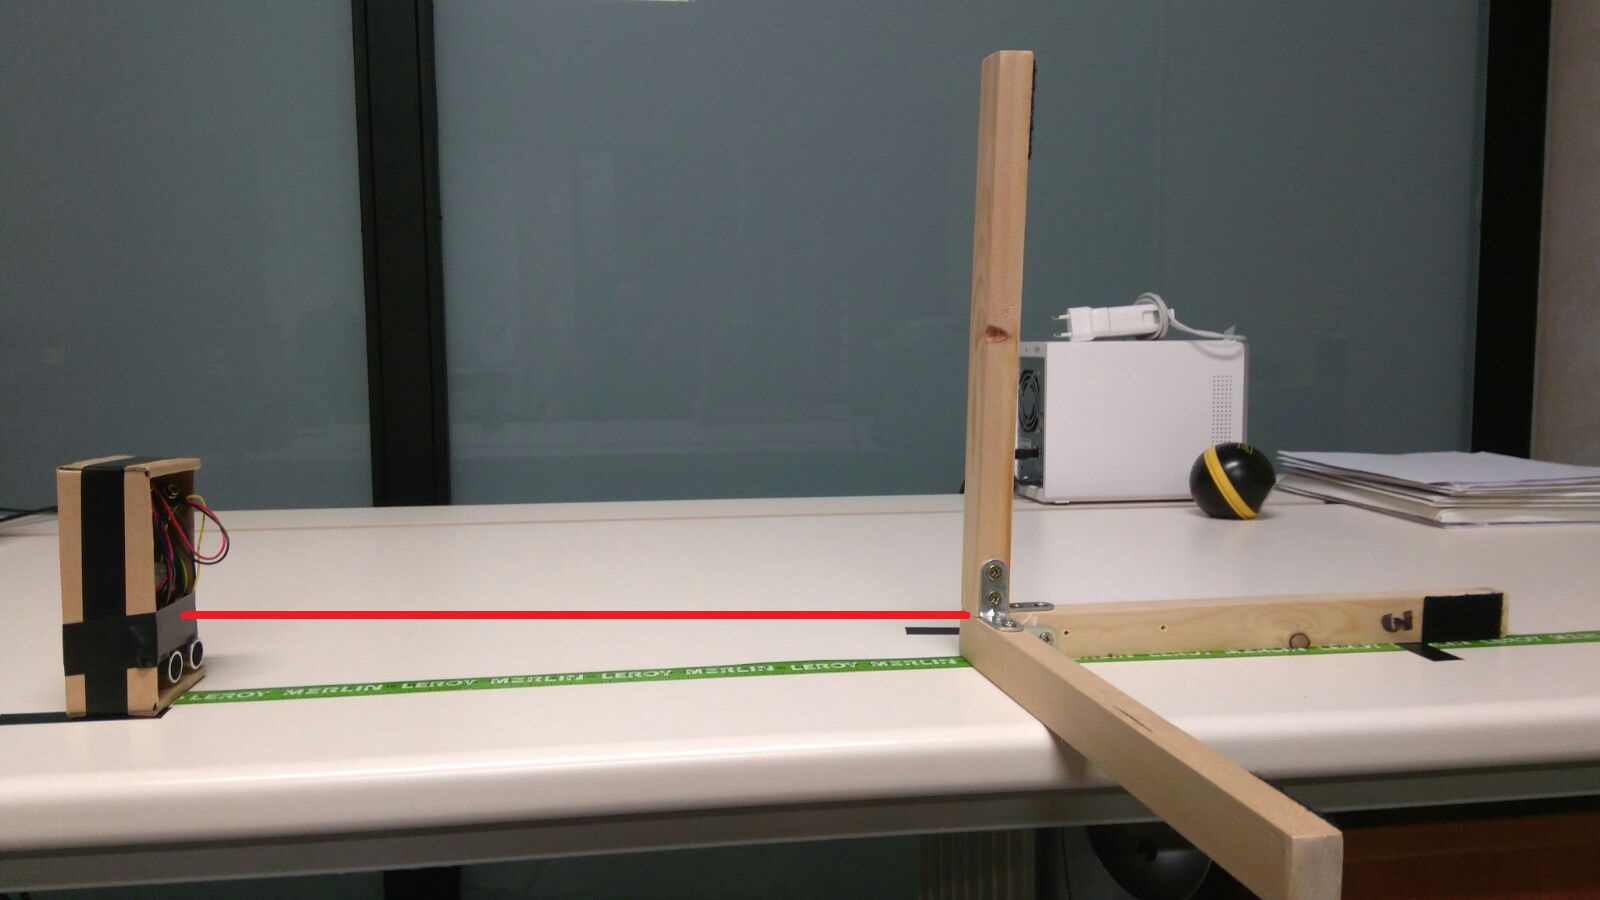
\includegraphics[width=0.95\textwidth]{./graphics/ultrasonido}
		 	\caption{Setup medida estática de sensor de ultrasonido}\label{fig:ultrasonido}
		 \end{figure}

Para estimar la precisión y el correcto funcionamiento del sensor se ha calculado el error absoluto y relativo de cada una de las medidas realizadas.

Una vez hecha dicha comprobación en estático, se añade al sistema de medida completo. Para ello se coloca el sensor en el tobillo y con el sensor orientado hacia la otra pierna (ver Figura \ref{fig:ultracoloc}).
		
	 \begin{figure}[H]
	 	\centering
	 	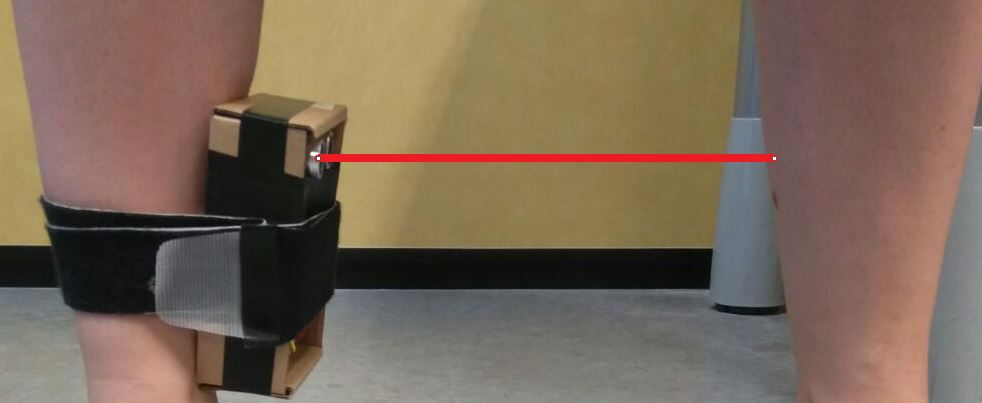
\includegraphics[width=0.8\textwidth]{./graphics/coloc_ultr}
	 	\caption{Colocación de sensor para medidas en dinámico} \label{fig:ultracoloc}
	 \end{figure}
				
		
\subsubsection{Obtención de distancia de separación entre pasos}

Una vez calculadas las distancias necesarias, se procede al cálculo de la distancia de separación entre pasos. En la Figura \ref{fig:sep} se representa dicho cálculo. La distancia D2 es la correspondiente al cálculo de la distancia con el sensor inercial izquierdo en este caso, la distancia D1 es la distancia calculada mediante el sensor de ultrasonido.
\begin{figure}[H]
	\centering
	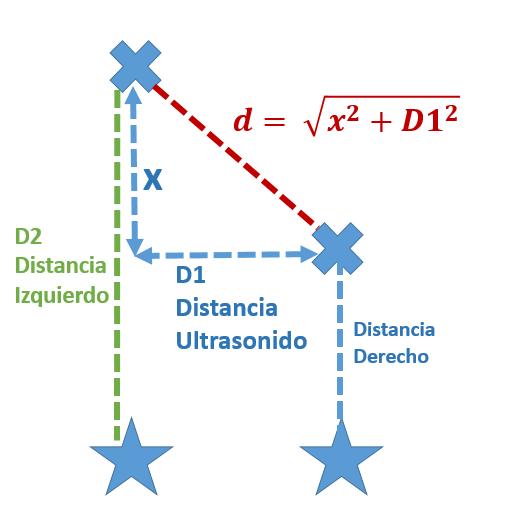
\includegraphics[width=0.8\textwidth]{./graphics/sep}
	\caption{Cálculo final de distancia de separación entre pasos} \label{fig:sep}
\end{figure}

Por tanto, para obtener X se utiliza la ecuación \ref{eq:x}
\begin{equation}\label{eq:x}
x = D2 - DistanciaDerecho
\end{equation}
En el caso de que el primero de los pasos se comenzase con el izquierdo la ecuación es la relativa a la DistanciaIzquierdo.

Para determinar la distancia, se utiliza por tanto, la ecuación \ref{eq:d}
\begin{equation}\label{eq:d}
d = \sqrt{x^{2}+D1^{2}}
\end{equation}